\documentclass{beamer}
\usepackage[utf8]{inputenc}
\usepackage{amsrefs, physics}
\usetheme{Frankfurt}
\usepackage{tikz-cd}
\usefonttheme[onlymath]{serif}

\title{CS 225 Final Project}
\author{Qianmeng Chen, Peilin He, Yikai Teng, Guangxun Zhai}
\institute{University of Illinois at Urbana-Champaign}
\date{\today}

\newtheorem*{claim}{Claim}
\newcommand{\mat}[1]{{\bf #1}}
\renewcommand{\vec}[1]{{\bf #1}}

\begin{document}

\frame{\titlepage}



\section{Goals}
\begin{frame}
\frametitle{Our goals} 
    \begin{block}{Leading Question}
        What is the most important airport around the world?
    \end{block}

    \begin{block}{Our Approach}
        The world's airline system can be viewed as a graph, with 
        \begin{itemize}
            \item Airports acting as nodes of the graph.
            \item Airlines (flights) acting as edges of the graph, and length of the flights acting as weights of edges.
        \end{itemize}
    \end{block}
    
    \begin{block}{Assumptions}
        \begin{itemize}
            \item The graph is undirected, since any flight has a corresponding return flight.
            \item The graph is ``irreflexive", meaning there is no flight taking off and landing at the same airport.
            \item The graph is simple, since two same fights can be seen as one.
        \end{itemize}
    \end{block}
\end{frame}



\begin{frame}
\frametitle{Accomplishments} 
    \begin{block}{Accomplishments}
        Within this project, we successfully accomplished the following:
        \begin{itemize}
            \item Read .dat files with given format as a graph.
            \item Traverse in the sense of breadth first search.
            \item Find a shortest path via Dijkstra Algorithm.
            \item Find a minimal spanning tree with Kruskal's Algorithm.
            \item Use page rank algorithm to determine which airport is the most inportant.
            \item Be able to visualize our result by rendering the graph to a ``world map" PNG file.
        \end{itemize}
    \end{block}
\end{frame}






\section{Development}

\begin{frame}
\frametitle{Airport, Airline, and the World}

\begin{block}{The Airport Class}
    An airport consists of an 3 or 4 letter abbreviation, and its coordinates on Earth. 
\end{block}

\begin{block}{The Airline Class}
    An airline consists of two pointers of airports, representing the source and destination, and a way to calculate the spherical distance between the two airports. 
\end{block}

\begin{block}{The world- the graph class}
    We use \textbf{Adjacent Matrices} to implement the graph because we do not need to change the number of airports a lot once we read the files.
\end{block}
    
\end{frame}



\begin{frame}
\frametitle{Processing .dat files}

\begin{block}{Overview}
    We need two .dat files, one for airports and the other for airlines. The data we use for this project comes from "openflights.org".
    
    In interpreting the data, if any broken data is observed, such as the latitude and longitude are NOT viable numbers, the corresponding entry will be neglected.
\end{block}

\begin{block}{A file for airports}
    The 3-letter, 4-letter abbr, latitudes, and longitudes are required to be in the 5th, 6th, 7th, 8th columns respectively.
\end{block}

\begin{block}{A file for airlines}
    The 3-letter or 4-letter abbr for the departing and arriving airports are required to be in the 3rd and 5th columns respectively.
\end{block}
    
\end{frame}


\begin{frame}
\frametitle{Traversal and Shortest Path}
\begin{block}{Traversal}
    BFS algorithm: \newline
    We built a void BFS function and a function that can return a vector saving all the traversing airports pointers. The overall codes for BFS followed the lectures: creating a list to record the status of whether being visited and a queue saving to deal with nodes and adjacent nodes.
\end{block}
\begin{block}{Shortest Path (Dijkstra's algorithm)}
    \begin{enumerate}
        \item Update the neighbor’s tentative distance value if we found a closer path.
        \item Put the neighbor into the priority queue. 
        \item Put the current node into the visited set.
    \end{enumerate} 
     
\end{block}
\end{frame}



\begin{frame}
\frametitle{MST}
\begin{block}{Kruskal's Minimum Spanning Tree}
    We built a Minimum Spanning tree by inserting edges in sorted order and keep the tree acyclic without any cycle. With Disjoint sets, we can keep track of nodes that are in the same connected components. This function returns a vector that contains all the airline pointer that has been traversed.
\end{block}
\begin{block}{Kruskal's Algorithm}
    \begin{enumerate}
        \item Sort the edges in increasing order of weights
        \item Initialize a separate disjoint set for each vertex
        \item For each edge uv, determine if they are in different sets
        \item If they are, add them to solution vector and union the sets
    \end{enumerate} 
\end{block}
\end{frame}


\begin{frame}
\frametitle{Page Rank}
\begin{block}{Helper Functions}
    \begin{itemize}
            \item Construct a matrix to store the value of our adjacent matrix. 
            \item Have a function to conduct matrix multiplication.
            \item Normalize the vector to prevent it from growing unlimited large.
        \end{itemize}
\end{block}
\begin{block}{Page Rank}
    We built a page rank function that can return a vector saving the results of our Markov Chain model. We count the number and quality of airline to a airport to determine a rough estimate of how important the airport is. This helps us to determine the most and top three important airports.
\end{block}
\end{frame}




\section{Analysis and Conclusions}
\begin{frame}

\frametitle{Running Time}
\begin{block}{BFS}
    $$O(n).$$
\end{block}

\begin{block}{ShortestPath (Dijkstra)}
    $$O(|E|+|V|\cdot ln(|V|)).$$
\end{block}

\begin{block}{MST (Kruskal)}
    $$O(m\cdot log(m)).$$
\end{block}

\begin{block}{Page Rank}
    $$O(n^2).$$
\end{block}

\end{frame}

\begin{frame}
\frametitle{Tests conducted}
\begin{block}{BFS Test Case}
    Firstly construct a simple tree graph and transverse through each nodes. The output is the traversal path. For this test, we check whether the airports saved in the path is following a BFS order.
\end{block}
\begin{block}{GetNeighbors Test Case}
    We also construct a simple graph with a node connected with several neighbor nodes. Then we tested whether this functions could return all the neighbor nodes in the graph.
\end{block}
\end{frame}

\begin{frame}
\frametitle{Tests conducted}
\begin{block}{ShortestPath Test Case}
    We created a graph that have different routes from the source node to the destination node. And we test for a specific source and destination, whether the shortest path between two nodes are the correct one.
\end{block}
\begin{block}{MST Test Case}
    A simple graph of 6 airports with 7 connected airlines is made. According to the distance between airports, we called MST to create a path of airports traversed with minimum weight. Then, we can check if the airports are correctly connected by edge weight. 
\end{block}
\end{frame}

\begin{frame}
\frametitle{Tests conducted}

\begin{block}{Page Rank Test Case}
    A simple graph of 7 airports with 5 connected airlines is made. According to the distance between airports, we called Findbest to find the most essential airport with the utilization of page rank. Then, we can check if the airports are correctly . 
\end{block}
\end{frame}

\begin{frame}
\frametitle{Some Visualizations}
\begin{block}{World Airports}
    Here is a plot of world airports (nodes of the graph). This also acts as a proof of the readFromFile works.
    \begin{center}
        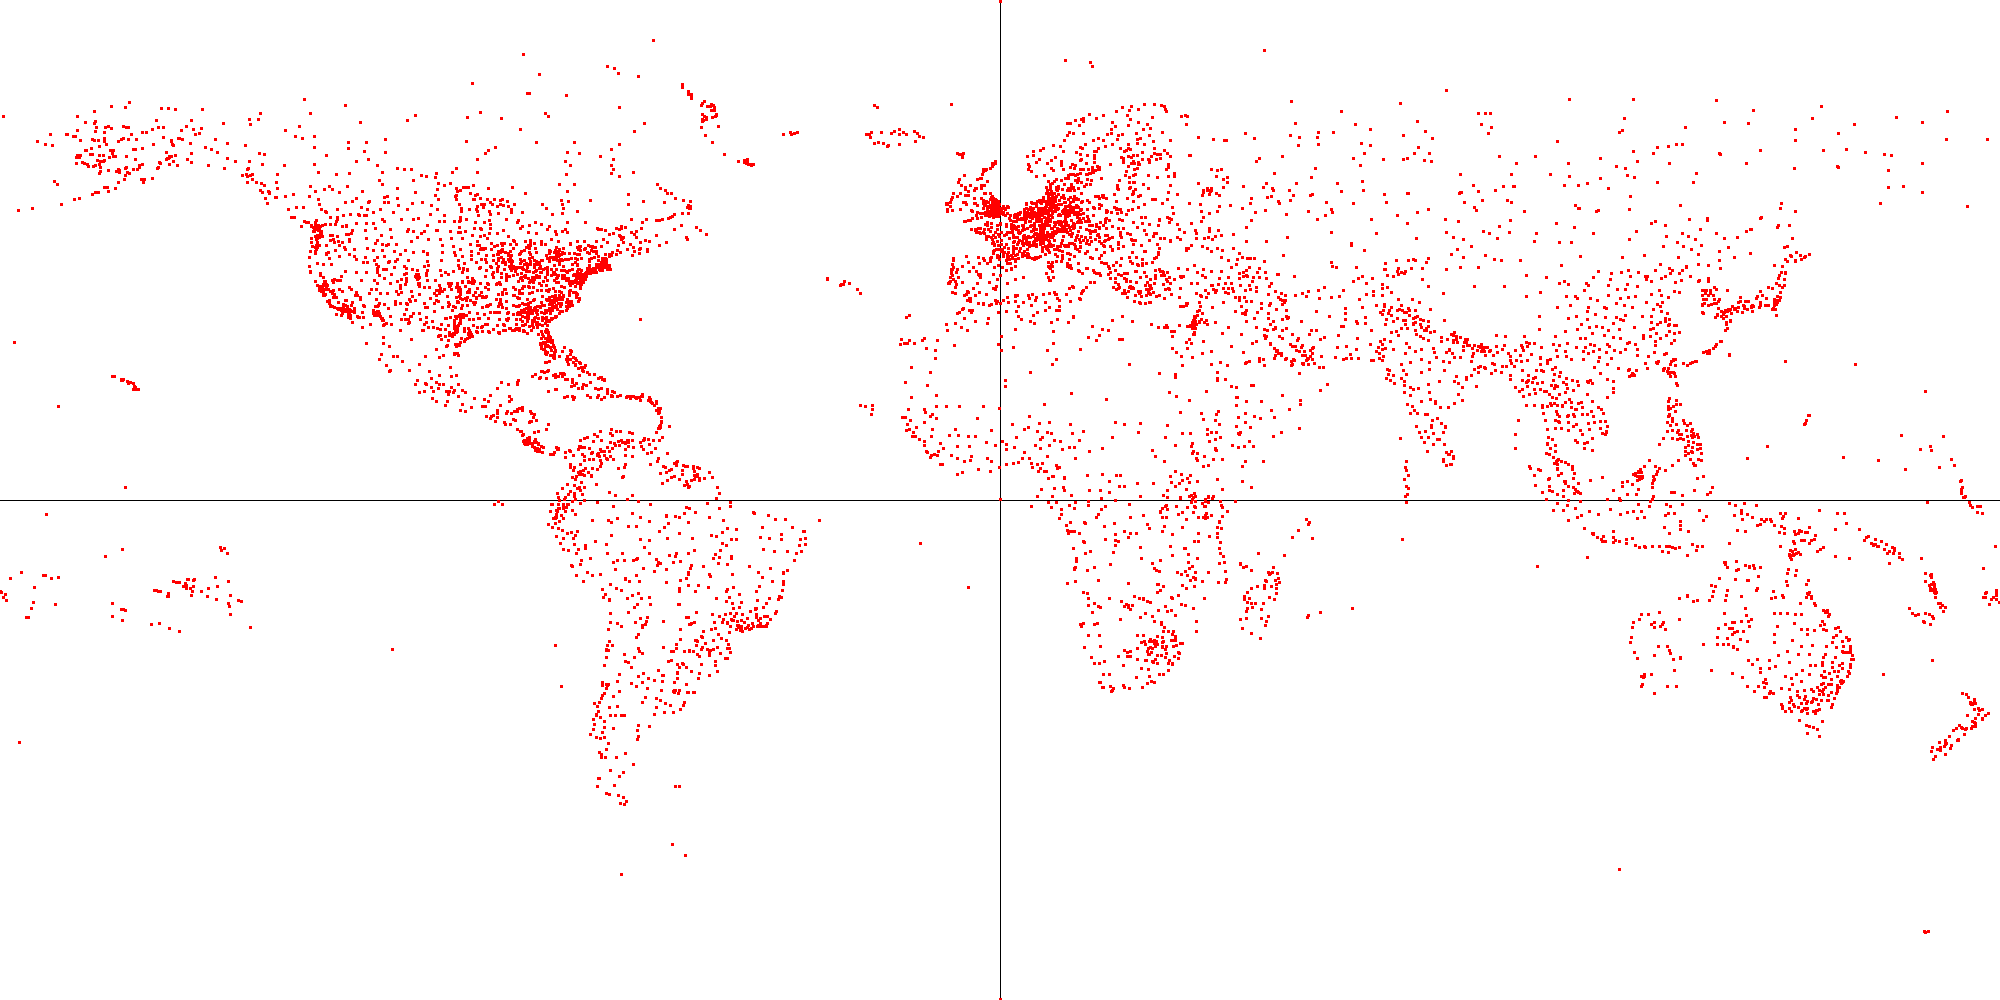
\includegraphics[width=10cm]{plots/world-airports.png}
    \end{center}
    
\end{block}
\end{frame}

\begin{frame}
\frametitle{Some Visualizations, cont.}
\begin{block}{World Airlines}
    Here is a plot of world airlines (edges of the graph). This also acts as a proof of the readFromFile works.
    \begin{center}
        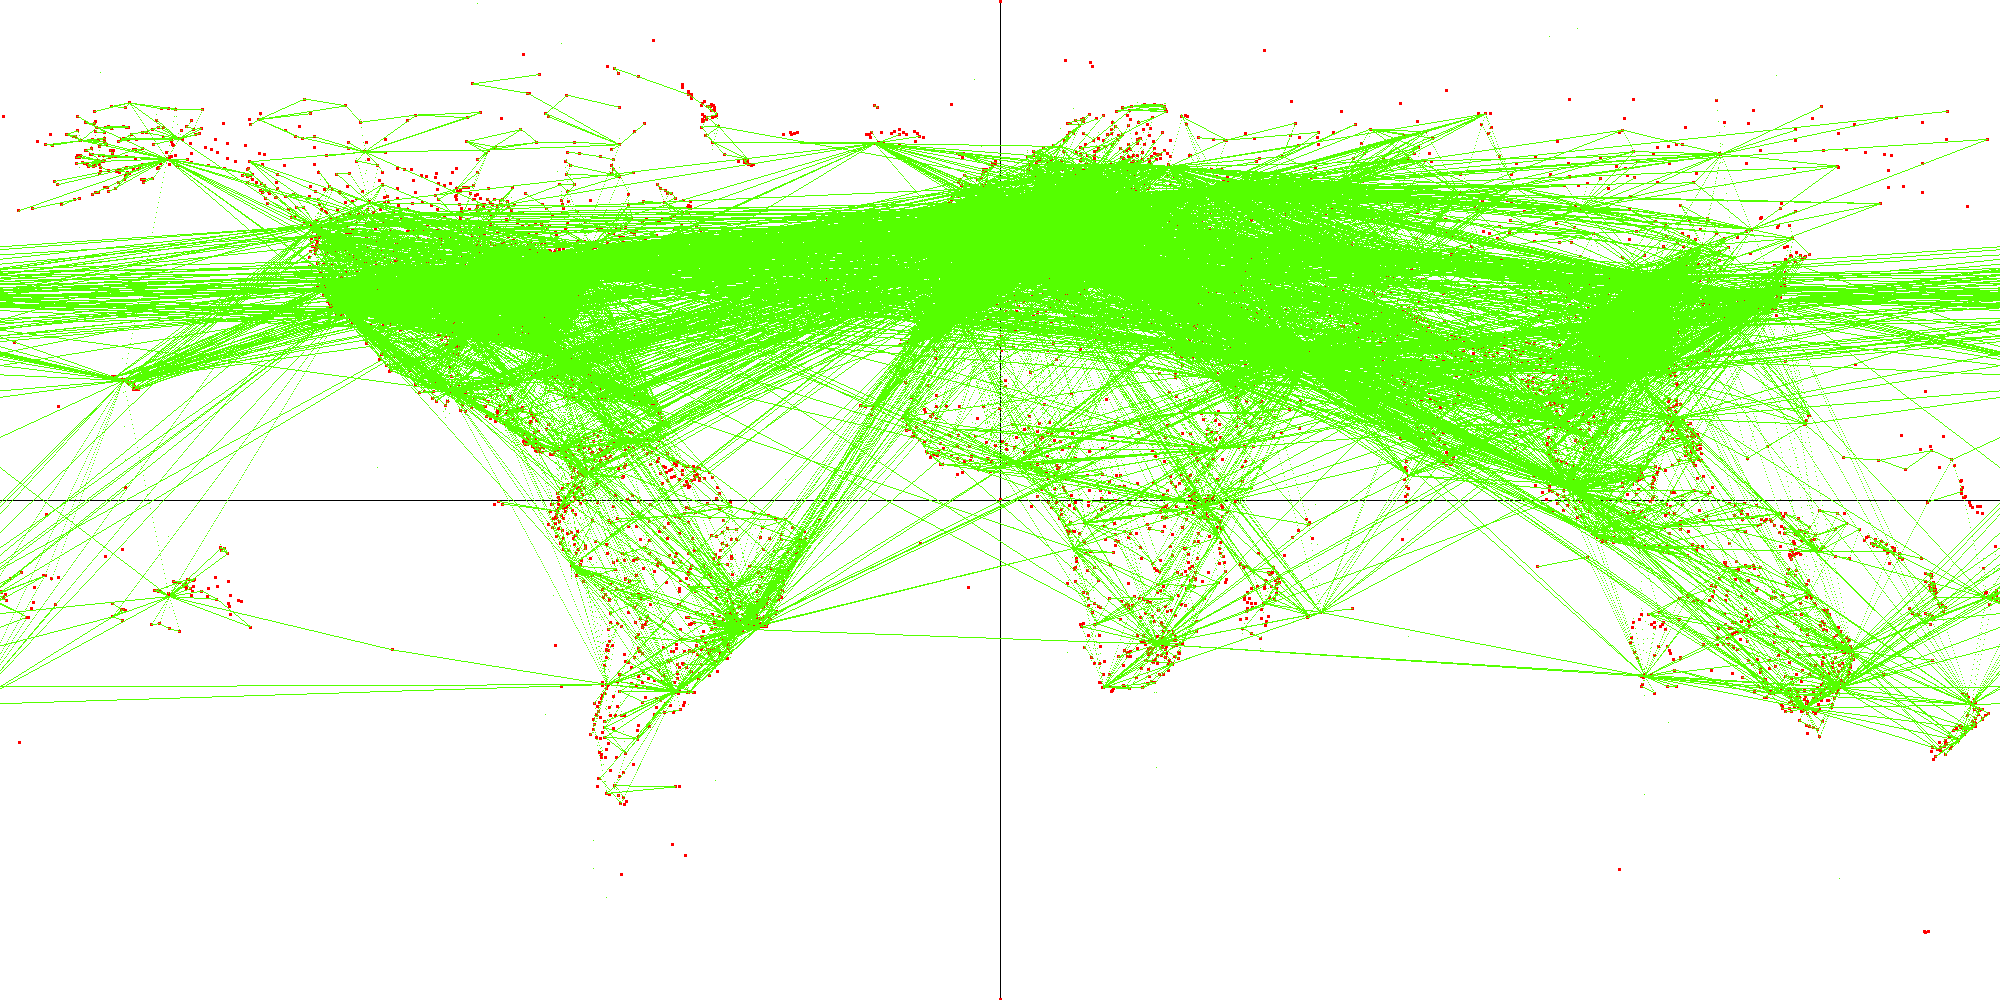
\includegraphics[width=10cm]{plots/world-airlines.png}
    \end{center}
    
\end{block}
\end{frame}

\begin{frame}
\frametitle{Some Visualizations, cont.}
\begin{block}{MST}
    Here is a plot of a minimal spanning tree drawn on top of world airlines. This also acts as a proof of the MST works.
    \begin{center}
        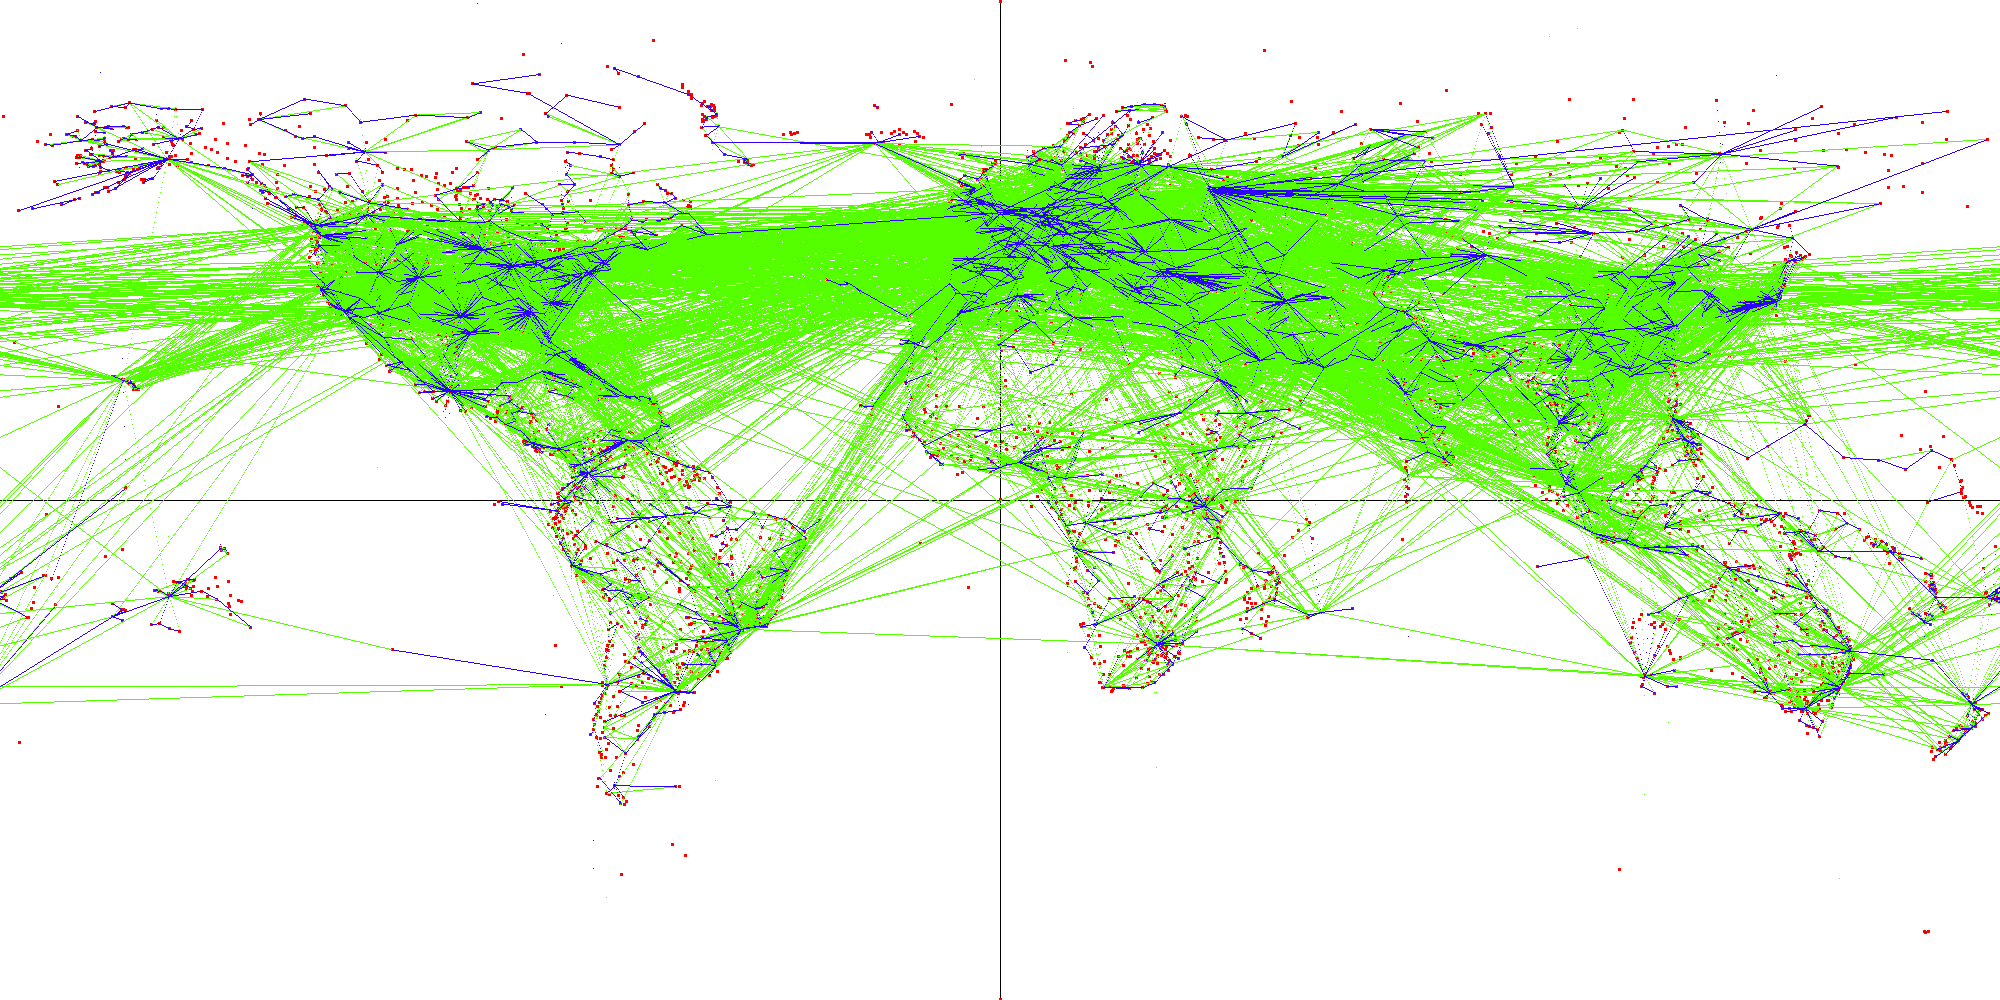
\includegraphics[width=10cm]{plots/MST.png}
    \end{center}
    
\end{block}
\end{frame}

\begin{frame}
\frametitle{Some Visualizations, cont.}
\begin{block}{Page Rank}
    Here is a plot of the top three most important airports worked out by Page Rank.
    \begin{center}
        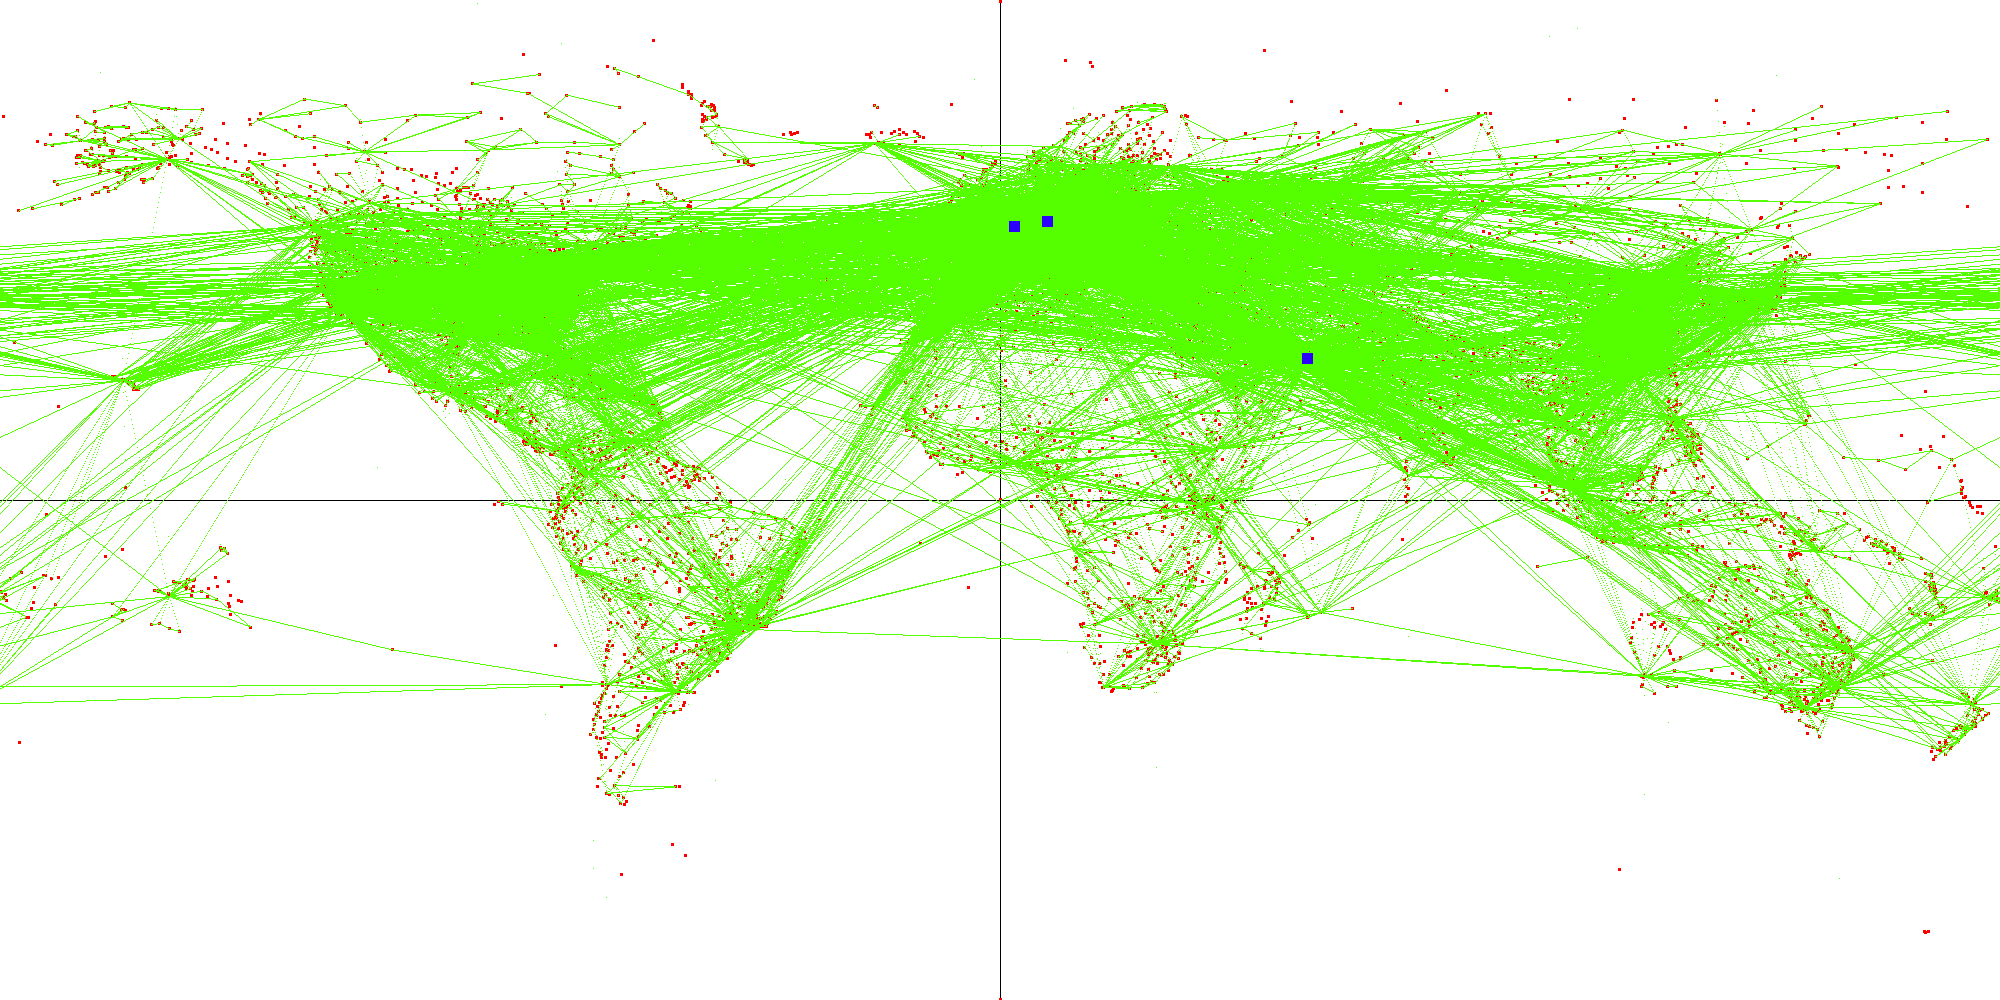
\includegraphics[width=10cm]{plots/top-three.png}
    \end{center}
    
\end{block}
\end{frame}

\begin{frame}
\frametitle{Answer to the leading question}
\begin{block}{Running time analysis}
    By running Page Rank algorithm, with distance between airports as weights, we have a ranking of all recorded airports in the world. The results are:
    \begin{itemize}
        \item The most important airport in the world is \textbf{FRA}, Frankfurt Airport in Germany.
        \item The second most important airport is \textbf{CDG}, Charles de Gaulle Airport in France.
        \item The third most important airport is \textbf{DXB}, Dubai International Airport in United Arab Emirates.
    \end{itemize}
\end{block}
\end{frame}



\end{document}